\begin{uzd}
Sąsiųvinyje per visą lapą nusibraižykite didelį stačiakampį padalintą į dalis kaip pavaizduota paveiksle.
Įrašykite žemiau pateiktus skaičius į siauriausią/mažiausią įmanomą skaičių aibę.
\begin{multicols}{7}
a) $0,33333 \ldots$

b) $-\frac{36}{12}$

c) $2,23606 \ldots$

d) $\sqrt{25}$

e) $51,(2)$

f) $6,43$

g) $\frac{20}{4}$

h) $0$

i) $\sqrt[3]{16}$

j) $\sqrt{1000}$

k) $\frac{10}{3}$

l) $\sqrt{15}$

m) $-28$

n) $\sqrt{\frac{4}{9}}$

o) $-\sqrt{81}$

p) $\pi$

q) $0.66 \ldots$

r) $-\frac{3}{12}$

s) $2,44948$

t) $1+\sqrt{2}$

u) $3.\overline{54}$

v) $1 \frac{2}{3}$

w) $-\frac{30}{6}$

x) $\sqrt[3]{125}$

y) $505$

z) $2 \pi$
\end{multicols}

\begin{center}
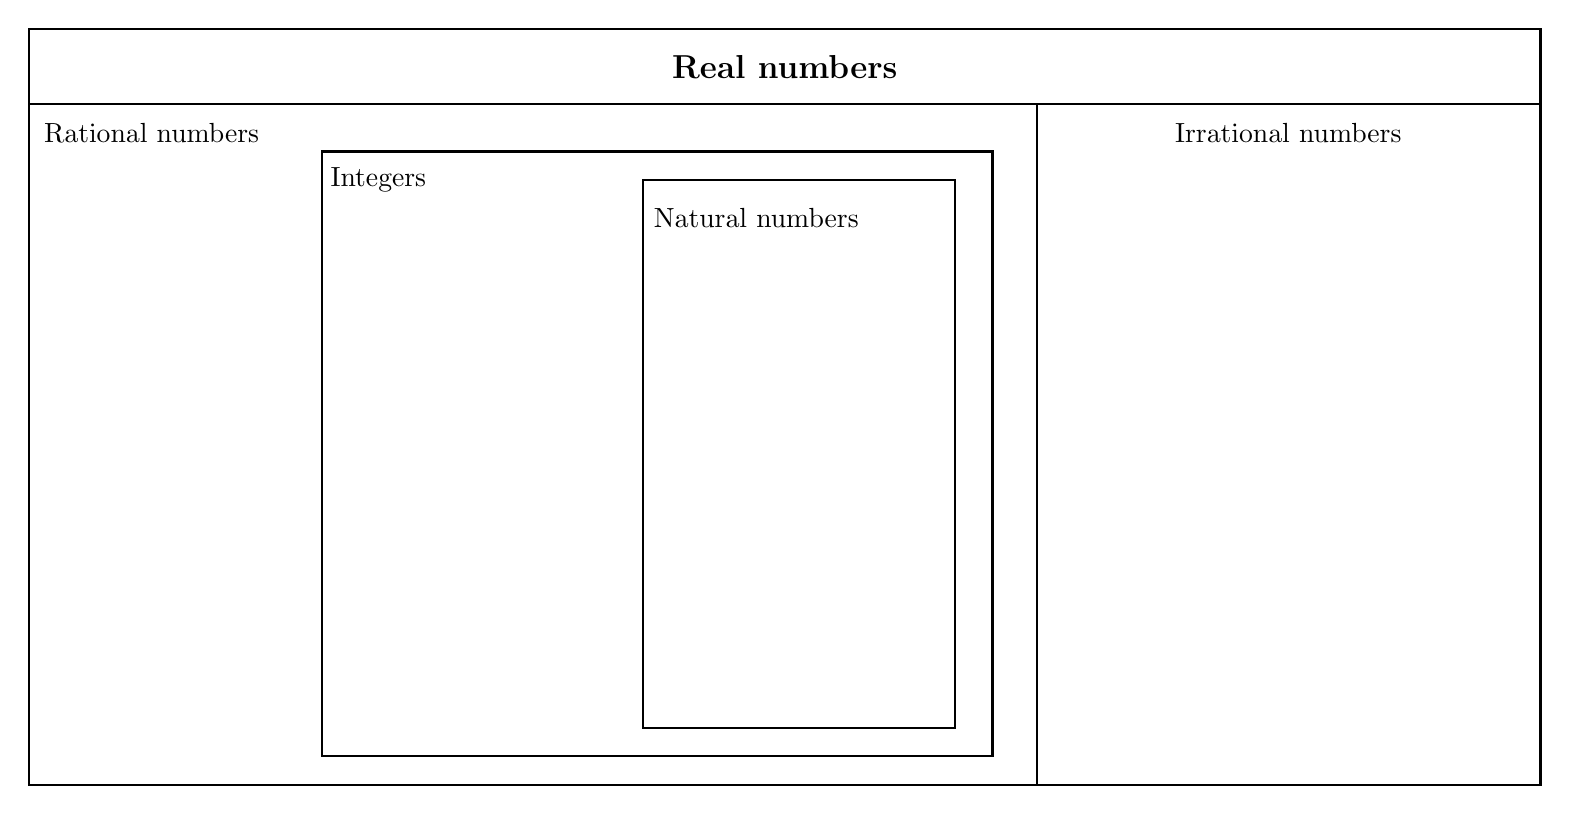
\begin{tikzpicture}[scale=1.2]
% Main rectangle - expanded to full page width
\draw[thick] (0,0) rectangle (16,8);

% Title at the top
\node[font=\large\bfseries] at (8,7.6) {Real numbers};

% Horizontal line below title
\draw[thick] (0,7.2) -- (16,7.2);

% Left section - Rational numbers
\draw[thick] (10.67,0) -- (10.67,7.2);
\node[font=\normalsize] at (1.3,6.9) {Rational numbers};

% Integers rectangle within Rational numbers
\draw[thick] (3.1,0.3) rectangle (10.2,6.7);
\node[font=\normalsize] at (3.7,6.4) {Integers};

% Natural numbers rectangle within Integers
\draw[thick] (6.5,0.6) rectangle (9.8,6.4);
\node[font=\normalsize] at (7.7,6) {Natural numbers};

% Right section - Irrational numbers  
\node[font=\normalsize] at (13.33,6.9) {Irrational numbers};
\end{tikzpicture}
\end{center}
\end{uzd}
\setcounter{teorema}{0}
\begin{uzd}
Sąsiųvinyje per visą lapą nusibraižykite didelį stačiakampį padalintą į dalis kaip pavaizduota paveiksle.
Įrašykite žemiau pateiktus skaičius į siauriausią/mažiausią įmanomą skaičių aibę.
\begin{multicols}{7}
a) $0,33333 \ldots$

b) $-\frac{36}{12}$

c) $2,23606 \ldots$

d) $\sqrt{25}$

e) $51,(2)$

f) $6,43$

g) $\frac{20}{4}$

h) $0$

i) $\sqrt[3]{16}$

j) $\sqrt{1000}$

k) $\frac{10}{3}$

l) $\sqrt{15}$

m) $-28$

n) $\sqrt{\frac{4}{9}}$

o) $-\sqrt{81}$

p) $\pi$

q) $0.66 \ldots$

r) $-\frac{3}{12}$

s) $2,44948$

t) $1+\sqrt{2}$

u) $3.\overline{54}$

v) $1 \frac{2}{3}$

w) $-\frac{30}{6}$

x) $\sqrt[3]{125}$

y) $505$

z) $2 \pi$
\end{multicols}

\begin{center}
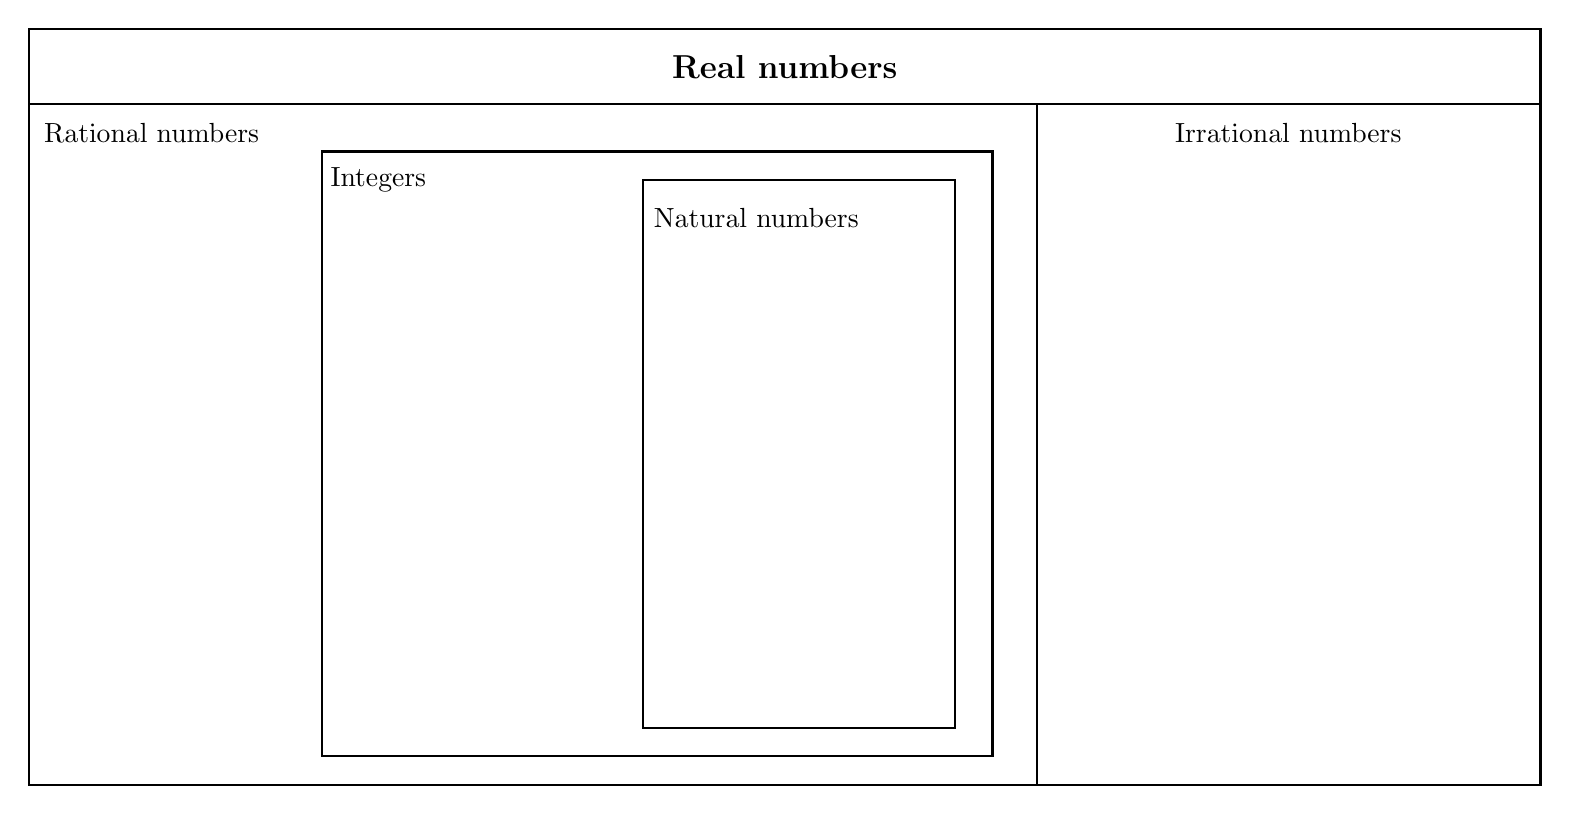
\begin{tikzpicture}[scale=1.2]
% Main rectangle - expanded to full page width
\draw[thick] (0,0) rectangle (16,8);

% Title at the top
\node[font=\large\bfseries] at (8,7.6) {Real numbers};

% Horizontal line below title
\draw[thick] (0,7.2) -- (16,7.2);

% Left section - Rational numbers
\draw[thick] (10.67,0) -- (10.67,7.2);
\node[font=\normalsize] at (1.3,6.9) {Rational numbers};

% Integers rectangle within Rational numbers
\draw[thick] (3.1,0.3) rectangle (10.2,6.7);
\node[font=\normalsize] at (3.7,6.4) {Integers};

% Natural numbers rectangle within Integers
\draw[thick] (6.5,0.6) rectangle (9.8,6.4);
\node[font=\normalsize] at (7.7,6) {Natural numbers};

% Right section - Irrational numbers  
\node[font=\normalsize] at (13.33,6.9) {Irrational numbers};
\end{tikzpicture}
\end{center}
\end{uzd}